\documentclass[aspectratio=169]{beamer}

% Theme and colors
\usetheme{Madrid}
\usecolortheme{whale}
\setbeamertemplate{navigation symbols}{}
\setbeamertemplate{footline}[frame number]

% Packages
\usepackage{tikz}
\usetikzlibrary{shapes,arrows,positioning,calc,decorations.pathreplacing}
\usepackage{booktabs}
\usepackage{graphicx}
\usepackage{xcolor}
\usepackage{tcolorbox}
\usepackage{array}

% Custom colors
\definecolor{aristotleblue}{RGB}{0,51,102}
\definecolor{techgray}{RGB}{64,64,64}
\definecolor{warningred}{RGB}{180,0,0}
\definecolor{virtuegreen}{RGB}{0,100,0}

% Custom blocks
\newtcolorbox{argumentbox}[1][]{
  colback=aristotleblue!5,
  colframe=aristotleblue,
  fonttitle=\bfseries,
  title={#1},
  boxrule=1pt,
  arc=2pt
}

\newtcolorbox{quotebox}[1][]{
  colback=gray!10,
  colframe=gray!50,
  fonttitle=\itshape,
  title={#1},
  boxrule=0.5pt,
  arc=2pt,
  left=10pt,
  right=10pt
}

\newtcolorbox{objectionbox}[1][]{
  colback=warningred!5,
  colframe=warningred,
  fonttitle=\bfseries,
  title={#1},
  boxrule=1pt,
  arc=2pt
}

% Title information
\title[Virtue Ethics \& Technology]{Virtue Ethics and Modern Technology}
\subtitle{Are Social Media and AI Making Us Stupider, Meaner, and Less Happy?}
\author{Brendan Shea, PhD}
\institute{Rochester Community and Technical College\\Computing and AI Ethics}
\date{}

\begin{document}

% ===== SLIDE 1: Title =====
\begin{frame}
\titlepage
\end{frame}

% ===== SLIDE 2: The Central Question =====
\begin{frame}{The Central Question}
\begin{itemize}
    \item Not just ``What should we do?'' but ``\textbf{What kind of people are we becoming?}''
    \item Technology isn't just a tool---it shapes our \textbf{character}
    \item Every swipe, click, and scroll is a form of \textbf{practice}
\end{itemize}

\vspace{0.5cm}
\begin{quotebox}[Aristotle, \textit{Nicomachean Ethics}]
``We are what we repeatedly do. Excellence, then, is not an act, but a habit.''
\end{quotebox}

\begin{alertblock}{?}
What technological habits have you developed in the last 5 years?
\end{alertblock}
\end{frame}

% ===== SLIDE 3: Introduction to Aristotle =====
\begin{frame}{Who Was Aristotle?}
\begin{columns}[T]
\column{0.5\textwidth}
\textbf{Life (384--322 BCE)}
\begin{itemize}
    \item Born in Stagira, northern Greece
    \item Studied at Plato's Academy for 20 years
    \item Tutor to Alexander the Great
    \item Founded his own school, the \textit{Lyceum}
\end{itemize}

\vspace{0.3cm}
\textbf{Revolutionary Thinker}
\begin{itemize}
    \item Focused on \textbf{observable nature}, not abstract forms
    \item Bridged theory and practice
    \item Founder of systematic logic
\end{itemize}

\column{0.5\textwidth}
\textbf{Why Aristotle?}
\begin{itemize}
    \item He asked: \textit{What is human flourishing?}
    \item He connected virtue to \textbf{habit and practice}
    \item His ethics are \textbf{deeply practical}---about how we actually live
    \item He understood that our \textbf{character is shaped} by repeated actions
\end{itemize}

\vspace{0.3cm}
\begin{alertblock}{The Key Insight}
Our character is not fixed. We \textit{become} virtuous through practice.
\end{alertblock}
\end{columns}
\end{frame}

% ===== SLIDE 4: Aristotle's Ethical Framework =====
\begin{frame}{Aristotle's Ethical Framework: The Big Picture}
\begin{itemize}
    \item Ethics as inquiry into the \textbf{good life} (not just right action)
    \item The \textbf{function argument} (\textit{ergon}): What is the distinctive function of human beings?
    \item \textbf{Virtue} (\textit{arête}) = excellence in performing our function
    \item Virtue leads to \textbf{flourishing} (\textit{eudaimonia})
\end{itemize}

\vspace{0.3cm}
\begin{center}
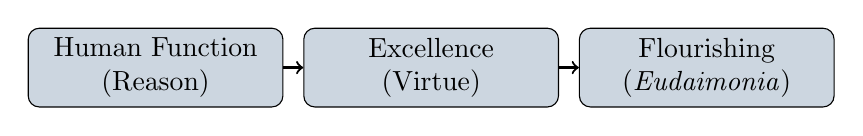
\begin{tikzpicture}[node distance=3.5cm, auto,
    block/.style={rectangle, draw, fill=aristotleblue!20, text width=3cm, text centered, rounded corners, minimum height=1cm}]
    \node [block] (function) {Human Function\\(Reason)};
    \node [block, right of=function] (excellence) {Excellence\\(Virtue)};
    \node [block, right of=excellence] (flourishing) {Flourishing\\(\textit{Eudaimonia})};
    \draw[->, thick] (function) -- (excellence);
    \draw[->, thick] (excellence) -- (flourishing);
\end{tikzpicture}
\end{center}
\end{frame}

% ===== SLIDE 5: Eudaimonia Defined =====
\begin{frame}{Eudaimonia Defined}
\begin{itemize}
    \item \textbf{Eudaimonia} = ``flourishing,'' ``well-being,'' ``living well and doing well''
    \item \textit{Not} ``happiness'' in the modern hedonic sense (feeling good)
    \item Activity of soul in accordance with virtue over a \textbf{complete life}
\end{itemize}

\vspace{0.3cm}
\begin{table}[h]
\centering
\small
\begin{tabular}{>{\bfseries}l p{3.5cm} p{3.5cm} p{3.5cm}}
\toprule
& \textbf{Eudaimonia} & \textbf{Hedonic Happiness} & \textbf{Life Satisfaction} \\
\midrule
Focus & Living virtuously & Feeling pleasure & Judging life positively \\
Timeframe & Complete life & Momentary & Retrospective \\
Source & Virtuous activity & Pleasant experiences & Meeting expectations \\
Can be wrong? & No (constitutive) & Yes (can feel happy doing bad) & Yes (can be mistaken) \\
\bottomrule
\end{tabular}
\end{table}
\end{frame}

% ===== SLIDE 6: The Nature of Virtue =====
\begin{frame}{The Nature of Virtue (\textit{Arête})}
\begin{itemize}
    \item Virtues are stable \textbf{character traits} (\textit{hexeis})
    \item The \textbf{Doctrine of the Mean}: Virtue as balance between excess and deficiency
    \item Virtues are \textbf{acquired through practice} and habituation
\end{itemize}

\vspace{0.5cm}
\begin{center}
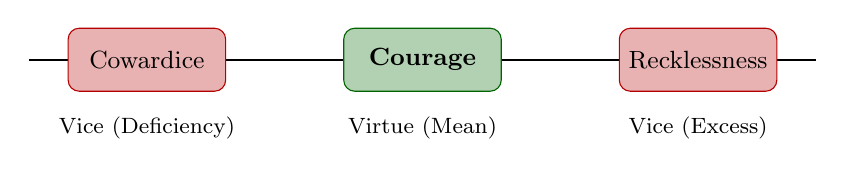
\begin{tikzpicture}
    % Draw the line
    \draw[thick, -] (0,0) -- (10,0);
    
    % Vice (deficiency)
    \node[fill=warningred!30, draw=warningred, rounded corners, minimum width=2cm, minimum height=0.8cm] at (1.5,0) {\small Cowardice};
    
    % Virtue (mean)
    \node[fill=virtuegreen!30, draw=virtuegreen, rounded corners, minimum width=2cm, minimum height=0.8cm] at (5,0) {\small \textbf{Courage}};
    
    % Vice (excess)
    \node[fill=warningred!30, draw=warningred, rounded corners, minimum width=2cm, minimum height=0.8cm] at (8.5,0) {\small Recklessness};
    
    % Labels
    \node[below] at (1.5,-0.6) {\footnotesize Vice (Deficiency)};
    \node[below] at (5,-0.6) {\footnotesize Virtue (Mean)};
    \node[below] at (8.5,-0.6) {\footnotesize Vice (Excess)};
\end{tikzpicture}
\end{center}

\begin{alertblock}{?}
Can you identify the mean between ``too much time spent online'' and ``too little''?
\end{alertblock}
\end{frame}

% ===== SLIDE 7: Intellectual vs. Moral Virtues =====
\begin{frame}{Intellectual vs. Moral Virtues}
\begin{columns}[T]
\begin{column}{0.48\textwidth}
\begin{block}{\textbf{Intellectual Virtues}}
\begin{itemize}
    \item \textbf{Sophia}: Theoretical wisdom
    \item \textbf{Phronesis}: Practical wisdom
    \item \textbf{Episteme}: Scientific knowledge
    \item \textbf{Nous}: Intuitive reason
    \item \textbf{Techne}: Craft/skill
\end{itemize}
\end{block}
\end{column}

\begin{column}{0.48\textwidth}
\begin{block}{\textbf{Moral Virtues}}
\begin{itemize}
    \item Courage
    \item Temperance
    \item Justice
    \item Generosity
    \item Honesty
    \item Friendliness
\end{itemize}
\end{block}
\end{column}
\end{columns}

\vspace{0.4cm}
\begin{alertblock}{Key Insight}
\textbf{Phronesis} (practical wisdom) is the ``master virtue''---it tells us how to apply all the other virtues in particular situations.
\end{alertblock}
\end{frame}

% ===== SLIDE 8: The Role of Phronesis =====
\begin{frame}{The Role of Phronesis (Practical Wisdom)}
\textbf{Phronesis} involves:
\begin{itemize}
    \item \textbf{Perception of particulars}: Seeing what the situation requires
    \item \textbf{Deliberation}: Reasoning about means to good ends
    \item \textbf{Integration}: Balancing competing considerations
    \item \textbf{Judgment}: Knowing when and how to act
\end{itemize}

\vspace{0.3cm}
\begin{center}
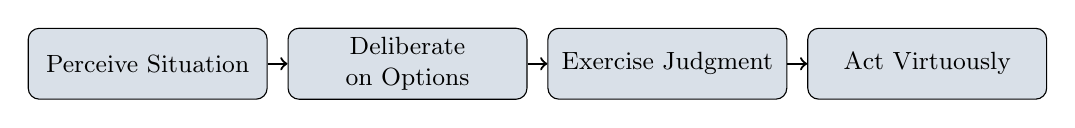
\begin{tikzpicture}[node distance=1.8cm,
    process/.style={rectangle, draw, fill=aristotleblue!15, text width=2.8cm, text centered, rounded corners, minimum height=0.9cm, font=\small}]
    \node [process] (perceive) {Perceive Situation};
    \node [process, right of=perceive, xshift=1.5cm] (deliberate) {Deliberate on Options};
    \node [process, right of=deliberate, xshift=1.5cm] (judge) {Exercise Judgment};
    \node [process, right of=judge, xshift=1.5cm] (act) {Act Virtuously};
    
    \draw[->, thick] (perceive) -- (deliberate);
    \draw[->, thick] (deliberate) -- (judge);
    \draw[->, thick] (judge) -- (act);
\end{tikzpicture}
\end{center}

\vspace{0.3cm}
\begin{alertblock}{Why This Matters for AI}
Phronesis \textit{cannot be reduced to rules or algorithms}---it requires human judgment shaped by experience and character.
\end{alertblock}
\end{frame}

% ===== SLIDE 9: Habituation and Moral Development =====
\begin{frame}{Habituation and Moral Development}
\begin{quotebox}[Aristotle]
``We become just by doing just acts, temperate by doing temperate acts, brave by doing brave acts.''
\end{quotebox}

\begin{itemize}
    \item Virtue requires \textbf{practice}---we learn by doing
    \item \textbf{Moral education} and environment matter enormously
\end{itemize}

\begin{center}
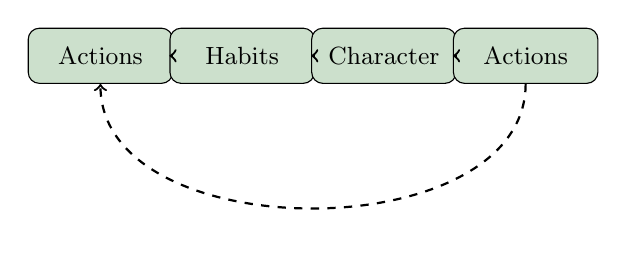
\begin{tikzpicture}[node distance=1.8cm,
    block/.style={rectangle, draw, fill=virtuegreen!20, text width=1.6cm, text centered, rounded corners, minimum height=0.7cm, font=\small}]
    \node [block] (actions) {Actions};
    \node [block, right of=actions] (habits) {Habits};
    \node [block, right of=habits] (character) {Character};
    \node [block, right of=character] (actions2) {Actions};
    \draw[->, thick] (actions) -- (habits);
    \draw[->, thick] (habits) -- (character);
    \draw[->, thick] (character) -- (actions2);
    \draw[->, thick, dashed] (actions2.south) to[out=-90,in=-90] (actions.south);
\end{tikzpicture}
\end{center}

\begin{alertblock}{?}
What character traits might daily social media use be cultivating in you?
\end{alertblock}
\end{frame}

% ===== SLIDE 10: Alasdair MacIntyre =====
\begin{frame}{Modern Revival: Alasdair MacIntyre}
\textbf{After Virtue} (1981): Diagnosis of moral fragmentation

\begin{itemize}
    \item \textbf{Emotivism critique}: Modern ethics lacks a shared framework
    \item Moral language has become ``masks for expressions of personal preference''
    \item Virtues require \textbf{social practices} and \textbf{traditions}
    \item We need \textbf{narrative unity}---understanding our lives as coherent stories
\end{itemize}

\vspace{0.3cm}
\begin{quotebox}[MacIntyre]
``I can only answer the question `What am I to do?' if I can answer the prior question `Of what story or stories do I find myself a part?'\,''
\end{quotebox}

\begin{alertblock}{?}
Does social media help or hinder you in constructing a coherent life narrative?
\end{alertblock}
\end{frame}

% ===== SLIDE 11: Rosalind Hursthouse =====
\begin{frame}{Modern Revival: Rosalind Hursthouse}
Virtue ethics \textit{is} action-guiding!

\begin{itemize}
    \item The \textbf{v-rules}: ``Do what is honest,'' ``Don't do what is cruel''
    \item Act as a \textbf{virtuous person} would act in the circumstances
    \item Virtue ethics handles \textbf{moral dilemmas} and ``moral residue''
\end{itemize}

\vspace{0.3cm}
\begin{table}[h]
\centering
\small
\begin{tabular}{>{\bfseries}l l l}
\toprule
& \textbf{Deontological Rules} & \textbf{V-Rules} \\
\midrule
Form & ``Don't lie'' & ``Be honest'' \\
Focus & Prohibited actions & Character \& motivation \\
Guidance & External constraints & Internal compass \\
Flexibility & Rigid application & Contextual wisdom \\
\bottomrule
\end{tabular}
\end{table}
\end{frame}

% ===== SLIDE 12: Martha Nussbaum =====
\begin{frame}{Modern Revival: Martha Nussbaum}
\textbf{Capabilities Approach}: What must humans be able to do/be to flourish?

\begin{itemize}
    \item Universal human \textbf{vulnerabilities and needs}
    \item Connects virtue ethics to \textbf{policy and social justice}
\end{itemize}

\vspace{0.2cm}
\begin{block}{Nussbaum's Central Capabilities (Selected)}
\footnotesize
\begin{enumerate}
    \item Life---living a life of normal length
    \item Bodily health---nourishment, shelter
    \item Senses, imagination, thought---education, free expression
    \item Emotions---attachments to things and people
    \item Practical reason---forming a conception of the good
    \item Affiliation---living with others, self-respect
    \item Play---recreational activities
\end{enumerate}
\end{block}

\begin{alertblock}{?}
Which of these capabilities might technology enhance? Which might it diminish?
\end{alertblock}
\end{frame}

% ===== SLIDE 13: Shannon Vallor =====
\begin{frame}{Shannon Vallor: Technology and the Virtues}
\textbf{Technomoral Virtues} for 21st-century flourishing:

\begin{itemize}
    \item We habituate ourselves \textit{through} our technological practices
    \item Technology can cultivate virtue \textit{or} vice
    \item Need a new framework for the digital age
\end{itemize}

\vspace{0.2cm}
\begin{block}{Vallor's Twelve Technomoral Virtues}
\begin{columns}[T]
\begin{column}{0.32\textwidth}
\small
\begin{itemize}
    \item Honesty
    \item Self-control
    \item Humility
    \item Justice
\end{itemize}
\end{column}
\begin{column}{0.32\textwidth}
\small
\begin{itemize}
    \item Courage
    \item Empathy
    \item Care
    \item Civility
\end{itemize}
\end{column}
\begin{column}{0.32\textwidth}
\small
\begin{itemize}
    \item Flexibility
    \item Perspective
    \item Magnanimity
    \item \textbf{Technomoral Wisdom}
\end{itemize}
\end{column}
\end{columns}
\end{block}
\end{frame}

% ===== PART II HEADER =====
\begin{frame}
\begin{center}
{\Huge \textbf{Part II}}\\[0.5cm]
{\Large Intellectual Virtues Under Threat}\\[0.3cm]
{\large Is Technology Making Us Stupider?}
\end{center}
\end{frame}

% ===== SLIDE 14: Intellectual Virtues Introduction =====
\begin{frame}{Intellectual Virtues at Stake}
Key \textbf{intellectual virtues} under examination:

\begin{columns}[T]
\begin{column}{0.48\textwidth}
\begin{itemize}
    \item \textbf{Curiosity}: Love of learning
    \item \textbf{Intellectual humility}: Recognizing limits
    \item \textbf{Love of truth}: Valuing accuracy over comfort
\end{itemize}
\end{column}
\begin{column}{0.48\textwidth}
\begin{itemize}
    \item \textbf{Open-mindedness}: Considering other views
    \item \textbf{Intellectual courage}: Following evidence
    \item \textbf{Intellectual autonomy}: Thinking for oneself
\end{itemize}
\end{column}
\end{columns}

\vspace{0.5cm}
\begin{alertblock}{The Central Question}
Are social media and AI systematically undermining our capacity to develop and exercise these virtues?
\end{alertblock}
\end{frame}

% ===== SLIDE 15: Argument in Standard Form (Intellectual) =====
\begin{frame}{Argument 1: Technology and Intellectual Vice}
\begin{argumentbox}[The Argument in Standard Form]
\begin{enumerate}
    \item Intellectual virtues are cultivated through sustained, effortful cognitive practices (attention, memory, critical analysis, deep reading).
    \item Social media and AI systematically replace or undermine these practices.
    \item Habituation in intellectually passive behaviors cultivates intellectual vice, not virtue.
    \item[\textbf{C.}] \textbf{Therefore, social media and AI tend to undermine intellectual virtue.}
\end{enumerate}
\end{argumentbox}

\vspace{0.3cm}
\textbf{Our task}: Examine the evidence for each premise.
\end{frame}

% ===== SLIDE 16: Premise 1 - How Intellectual Virtues Are Cultivated =====
\begin{frame}{Premise 1: How Intellectual Virtues Are Cultivated}
Intellectual virtue requires \textbf{effortful practice}:

\begin{itemize}
    \item Develop \textbf{sustained attention} through deep reading and focused study
    \item Engage in \textbf{memory work} through effortful encoding and retrieval
    \item Practice \textbf{confronting difficulty} by struggling without immediate help
    \item Seek \textbf{diverse exposure} by encountering challenging viewpoints
    \item Cultivate \textbf{slow thinking} through deliberate reasoning over snap judgments
\end{itemize}

\vspace{0.3cm}
\begin{quotebox}[William James]
``The faculty of voluntarily bringing back a wandering attention, over and over again, is the very root of judgment, character, and will.''
\end{quotebox}
\end{frame}

% ===== SLIDE 17: Premise 2a - The Attention Crisis =====
\begin{frame}{Premise 2a: The Attention Crisis}
\textbf{Nicholas Carr}, \textit{The Shallows} (2010) and \textbf{Jonathan Haidt}:

\begin{itemize}
    \item Internet use literally \textbf{rewires the brain} for distraction
    \item \textbf{Variable reward schedules} hijack dopamine systems
    \item ``\textbf{Continuous partial attention}'' replaces deep focus
    \item Average time on task before switching: declining steadily
\end{itemize}

\vspace{0.3cm}
\begin{table}[h]
\centering
\small
\begin{tabular}{l c c}
\toprule
\textbf{Metric} & \textbf{2004} & \textbf{2024} \\
\midrule
Avg. attention span on screens & 2.5 minutes & 47 seconds \\
Deep reading time (teens) & 60 min/day & 15 min/day \\
Phone checks per day & N/A & 150+ times \\
\bottomrule
\end{tabular}
\caption{\small Approximate figures from attention research}
\end{table}

\begin{alertblock}{?}
When was the last time you read for 30+ minutes without checking your phone?
\end{alertblock}
\end{frame}

% ===== SLIDE 18: Premise 2b - Outsourcing Memory =====
\begin{frame}{Premise 2b: Outsourcing Memory and Cognition}
\textbf{Cognitive offloading}: Using technology as external memory

\begin{itemize}
    \item The \textbf{``Google Effects on Memory''} (Sparrow et al., 2011) shows we remember \textit{where} to find information rather than the information itself
    \item \textbf{GPS navigation} reduces spatial reasoning and mental mapping
    \item \textbf{AI writing tools} outsource composition and critical thinking
    \item \textbf{Calculators and now AI} deepen the deskilling concern beyond simple math
\end{itemize}

\vspace{0.3cm}
\begin{alertblock}{The Concern}
If we don't \textit{practice} remembering, analyzing, and reasoning, we don't develop the intellectual virtues that these activities cultivate.
\end{alertblock}
\end{frame}

% ===== SLIDE 19: Premise 2c - Echo Chambers =====
\begin{frame}{Premise 2c: Epistemic Bubbles and Echo Chambers}
\textbf{C. Thi Nguyen's} important distinction:

\begin{table}[h]
\centering
\small
\begin{tabular}{>{\bfseries}l p{4.5cm} p{4.5cm}}
\toprule
& \textbf{Epistemic Bubble} & \textbf{Echo Chamber} \\
\midrule
Mechanism & Other voices not heard & Other voices actively discredited \\
Result & Missing information & Distrust of outside sources \\
Fix & Exposure to other views & Much harder---trust must be rebuilt \\
\bottomrule
\end{tabular}
\end{table}

\vspace{0.2cm}
\begin{itemize}
    \item \textbf{Algorithmic curation} creates bubbles by design
    \item Engagement-maximizing algorithms reward \textbf{confirmation bias}
    \item Undermines \textbf{intellectual humility} and \textbf{open-mindedness}
\end{itemize}

\begin{alertblock}{?}
How often do you seek out viewpoints that challenge your own beliefs?
\end{alertblock}
\end{frame}

% ===== SLIDE 20: Premise 2d - AI and Intellectual Dependency =====
\begin{frame}{Premise 2d: AI and Intellectual Dependency}
\textbf{Shannon Vallor} on ``moral deskilling'' through automation:

\begin{itemize}
    \item ChatGPT and the \textbf{outsourcing of thinking itself}
    \item Parallel to calculator debates---but \textit{much deeper}
    \item We lose the \textbf{struggle} that builds intellectual virtue
    \item AI provides answers without cultivating \textbf{understanding}
\end{itemize}

\vspace{0.3cm}
\begin{quotebox}[Vallor, \textit{Technology and the Virtues}]
``Technologies that remove the need for us to develop or exercise our own practical skills and judgment \ldots\ can weaken or even eliminate our opportunities to cultivate virtue.''
\end{quotebox}

\begin{alertblock}{?}
When is it appropriate to use AI for help vs. when does it become intellectual ``cheating''?
\end{alertblock}
\end{frame}

% ===== SLIDE 21: Synthesis - Intellectual Virtues =====
\begin{frame}{Synthesis: Intellectual Virtue Undermined}
\begin{center}
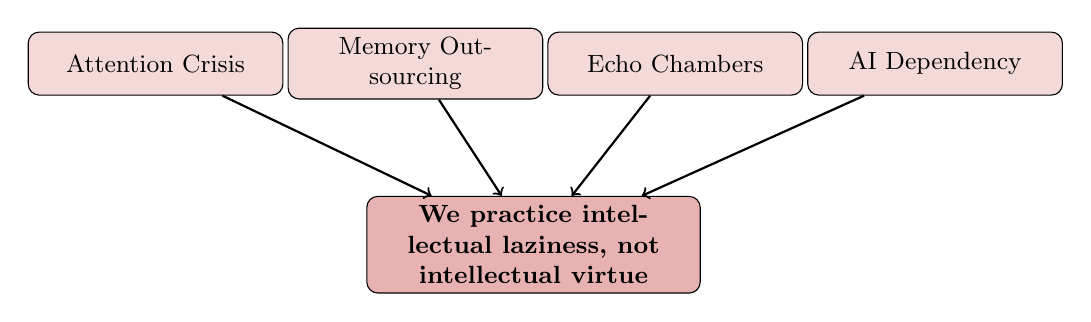
\begin{tikzpicture}[node distance=1.5cm,
    evidence/.style={rectangle, draw, fill=warningred!15, text width=3cm, text centered, rounded corners, minimum height=0.8cm, font=\small},
    result/.style={rectangle, draw, fill=warningred!30, text width=4cm, text centered, rounded corners, minimum height=1cm, font=\small\bfseries}]
    
    \node [evidence] (attention) {Attention Crisis};
    \node [evidence, right of=attention, xshift=1.8cm] (memory) {Memory Outsourcing};
    \node [evidence, right of=memory, xshift=1.8cm] (echo) {Echo Chambers};
    \node [evidence, right of=echo, xshift=1.8cm] (ai) {AI Dependency};
    
    \node [result, below of=memory, xshift=1.5cm, yshift=-0.8cm] (conclusion) {We practice intellectual laziness, not intellectual virtue};
    
    \draw[->, thick] (attention) -- (conclusion);
    \draw[->, thick] (memory) -- (conclusion);
    \draw[->, thick] (echo) -- (conclusion);
    \draw[->, thick] (ai) -- (conclusion);
\end{tikzpicture}
\end{center}

\vspace{0.3cm}
\textbf{Connecting back to Aristotle}: We become what we repeatedly do. If we repeatedly practice distraction, outsourcing, and intellectual passivity, we cultivate intellectual \textit{vice}.
\end{frame}

% ===== PART III HEADER =====
\begin{frame}
\begin{center}
{\Huge \textbf{Part III}}\\[0.5cm]
{\Large Moral Virtues Under Threat}\\[0.3cm]
{\large Is Technology Making Us Meaner?}
\end{center}
\end{frame}

% ===== SLIDE 21: Moral Virtues Introduction =====
\begin{frame}{Moral Virtues at Stake}
Key \textbf{moral virtues} under examination:

\begin{columns}[T]
\begin{column}{0.48\textwidth}
\begin{itemize}
    \item \textbf{Empathy}: Feeling with others
    \item \textbf{Compassion}: Caring about suffering
    \item \textbf{Patience}: Tolerating delay/difficulty
    \item \textbf{Temperance}: Self-control
\end{itemize}
\end{column}
\begin{column}{0.48\textwidth}
\begin{itemize}
    \item \textbf{Civility}: Respectful discourse
    \item \textbf{Honesty}: Truthfulness
    \item \textbf{Justice}: Fairness to others
    \item \textbf{Kindness}: Benevolence
\end{itemize}
\end{column}
\end{columns}

\vspace{0.5cm}
\begin{alertblock}{The Central Question}
Are social media and AI systematically undermining our capacity to develop and exercise these virtues?
\end{alertblock}
\end{frame}

% ===== SLIDE 22: Argument in Standard Form (Moral) =====
\begin{frame}{Argument 2: Technology and Moral Vice}
\begin{argumentbox}[The Argument in Standard Form]
\begin{enumerate}
    \item Moral virtues are cultivated through embodied, face-to-face social practices involving vulnerability and reciprocity.
    \item Digital mediation systematically degrades or replaces these practices.
    \item Online environments actively habituate us toward moral vices (cruelty, impatience, dishonesty, outrage).
    \item[\textbf{C.}] \textbf{Therefore, social media and AI tend to undermine moral virtue.}
\end{enumerate}
\end{argumentbox}

\vspace{0.3cm}
\textbf{Our task}: Examine the evidence for each premise.
\end{frame}

% ===== SLIDE 23: Premise 1 - Turkle on Conversation =====
\begin{frame}{Premise 1: How Moral Virtues Are Cultivated}
\textbf{Sherry Turkle}, \textit{Reclaiming Conversation} (2015):

\begin{itemize}
    \item \textbf{Face-to-face conversation} is the crucible of empathy
    \item We need \textbf{embodied presence}---eye contact, tone, physical co-presence
    \item Moral development requires \textbf{vulnerability and reciprocity}
    \item Learning to tolerate \textbf{boredom and discomfort} builds character
\end{itemize}

\vspace{0.3cm}
\begin{quotebox}[Turkle]
``Face-to-face conversation is the most human---and humanizing---thing we do. Fully present to one another, we learn to listen. It's where we develop the capacity for empathy.''
\end{quotebox}

\begin{alertblock}{?}
Do you behave differently in text messages than in face-to-face conversation? How?
\end{alertblock}
\end{frame}

% ===== SLIDE 24: Premise 2a - Empathy Decline =====
\begin{frame}{Premise 2a: The Empathy Decline}
\textbf{University of Michigan meta-study} (Konrath et al., 2011):

\begin{itemize}
    \item \textbf{40\% decline} in empathy among college students (1979--2009)
    \item Steepest decline after 2000---correlates with digital communication rise
    \item Teens spending less time in \textbf{face-to-face interaction}
    \item Empathy requires \textbf{practice}---and we're practicing less
\end{itemize}

\vspace{0.3cm}
\begin{center}
\begin{tikzpicture}
    \draw[->] (0,0) -- (8,0) node[right] {\small Year};
    \draw[->] (0,0) -- (0,3) node[above] {\small Empathy};
    \draw[thick, warningred] (0.5,2.5) -- (3,2.3) -- (5,1.8) -- (7.5,1.5);
    \node[below] at (0.5,0) {\tiny 1979};
    \node[below] at (3,0) {\tiny 1990};
    \node[below] at (5,0) {\tiny 2000};
    \node[below] at (7.5,0) {\tiny 2009};
    \draw[dashed] (5,0) -- (5,1.8);
    \node[right, font=\tiny] at (5.1,0.9) {Steeper decline};
\end{tikzpicture}
\end{center}
\end{frame}

% ===== SLIDE 25: Premise 2b - Online Disinhibition =====
\begin{frame}{Premise 2b: Online Disinhibition and Cruelty}
\textbf{John Suler's} ``Online Disinhibition Effect'':

\begin{table}[h]
\centering
\small
\begin{tabular}{>{\bfseries}l p{7cm}}
\toprule
Factor & Effect on Behavior \\
\midrule
Anonymity & ``You don't know me''---reduced accountability \\
Invisibility & Can't see victim's pain---reduced empathy cues \\
Asynchronicity & No immediate feedback---say things you'd regret \\
Dissociative imagination & Online self feels separate from ``real'' self \\
Minimization of authority & Flattened hierarchies, less restraint \\
\bottomrule
\end{tabular}
\end{table}

\vspace{0.2cm}
\begin{alertblock}{Result}
The normalization of cruelty: Behaviors that would be unthinkable in person become routine online.
\end{alertblock}

\begin{alertblock}{?}
Have you ever posted something online you wouldn't say to someone's face?
\end{alertblock}
\end{frame}

% ===== SLIDE 26: Premise 2c - Outrage as Business Model =====
\begin{frame}{Premise 2c: Outrage as Business Model}
\textbf{Jonathan Haidt} on social media's transformation:

\begin{itemize}
    \item \textbf{2009}: Facebook adds ``Like''; Twitter adds ``Retweet''
    \item \textbf{Outrage generates engagement}---anger spreads faster than joy
    \item \textbf{Moral grandstanding} rewarded over moral action
    \item \textbf{Tribal epistemology}: Demonization of the ``other side''
\end{itemize}

\begin{center}
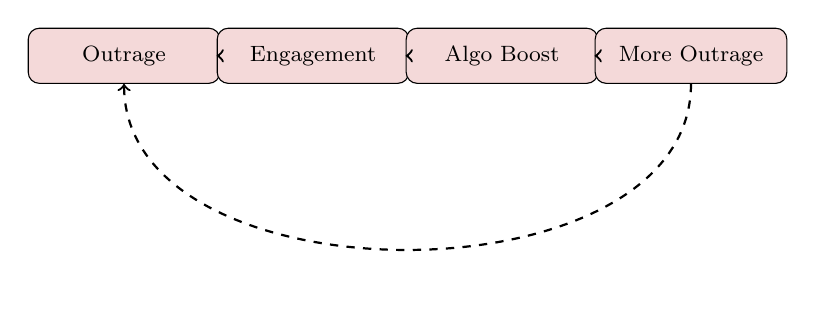
\begin{tikzpicture}[node distance=1.8cm,
    block/.style={rectangle, draw, fill=warningred!15, text width=2.2cm, text centered, rounded corners, minimum height=0.7cm, font=\footnotesize}]
    \node [block] (content) {Outrage};
    \node [block, right of=content, xshift=0.6cm] (engagement) {Engagement};
    \node [block, right of=engagement, xshift=0.6cm] (algorithm) {Algo Boost};
    \node [block, right of=algorithm, xshift=0.6cm] (more) {More Outrage};
    \draw[->, thick] (content) -- (engagement);
    \draw[->, thick] (engagement) -- (algorithm);
    \draw[->, thick] (algorithm) -- (more);
    \draw[->, thick, dashed] (more.south) to[out=-90,in=-90] (content.south);
\end{tikzpicture}
\end{center}

\begin{alertblock}{?}
Have you ever shared something online primarily because it made you angry?
\end{alertblock}
\end{frame}

% ===== SLIDE 27: Premise 2d - Dishonesty and Performance =====
\begin{frame}{Premise 2d: Dishonesty and Performative Identity}
Technology enables and encourages \textbf{inauthenticity}:

\begin{itemize}
    \item \textbf{Curated self-presentation} creates a gap between Instagram and reality
    \item \textbf{Performative virtue} allows us to signal goodness without actually being good
    \item \textbf{Deepfakes and synthetic media} make truth increasingly optional
    \item \textbf{AI-generated content} erodes authentic human communication
    \item These combine to cause a \textbf{collapse of trust} in media, institutions, and each other
\end{itemize}

\vspace{0.3cm}
\begin{quotebox}[Hannah Arendt]
``The ideal subject of totalitarian rule is not the convinced Nazi or the convinced Communist, but people for whom the distinction between fact and fiction \ldots\ no longer exists.''
\end{quotebox}
\end{frame}

% ===== SLIDE 28: Synthesis - Moral Virtues =====
\begin{frame}{Synthesis: Moral Virtue Undermined}
\begin{table}[h]
\centering
\small
\begin{tabular}{>{\bfseries}l l l}
\toprule
Virtue & Traditional Practice & Digital Replacement \\
\midrule
Empathy & Face-to-face conversation & Text-based interaction \\
Patience & Waiting, delayed gratification & Instant everything \\
Civility & Social norms, accountability & Anonymous cruelty \\
Honesty & Reputation, trust-building & Curated personas \\
Temperance & Natural limits & Infinite scroll, autoplay \\
\bottomrule
\end{tabular}
\end{table}

\vspace{0.3cm}
\begin{alertblock}{The Habituation Problem}
We are practicing outrage instead of empathy, cruelty instead of kindness, performance instead of authenticity. \textbf{We become what we practice.}
\end{alertblock}

\begin{alertblock}{?}
What emotions does your social media feed most often evoke in you?
\end{alertblock}
\end{frame}

% ===== PART IV HEADER =====
\begin{frame}
\begin{center}
{\Huge \textbf{Part IV}}\\[0.5cm]
{\Large Eudaimonia Under Threat}\\[0.3cm]
{\large Is Technology Making Us Less Happy?}
\end{center}
\end{frame}

% ===== SLIDE 29: Eudaimonia Introduction =====
\begin{frame}{Eudaimonia Under Threat}
Beyond individual virtues: the \textbf{whole flourishing life}

\begin{itemize}
    \item Eudaimonia requires \textbf{integrated exercise of virtue} across a complete life
    \item It requires \textbf{meaningful relationships}, not just connections
    \item It requires \textbf{purposeful activity}, not just consumption
    \item It requires \textbf{self-knowledge}, not algorithmic identity
\end{itemize}

\vspace{0.4cm}
\begin{alertblock}{Important Note}
``Happiness'' here means \textit{eudaimonia}---not just feeling good, but genuinely flourishing as a human being.
\end{alertblock}
\end{frame}

% ===== SLIDE 30: Argument in Standard Form (Eudaimonia) =====
\begin{frame}{Argument 3: Technology and Diminished Flourishing}
\begin{argumentbox}[The Argument in Standard Form]
\begin{enumerate}
    \item Eudaimonia requires integrated exercise of virtue across a complete life, including meaningful relationships, purposeful activity, and self-knowledge.
    \item Social media and AI fragment attention, commodify relationships, and distort self-understanding.
    \item These effects directly impede the conditions necessary for eudaimonia.
    \item[\textbf{C.}] \textbf{Therefore, social media and AI tend to undermine human flourishing.}
\end{enumerate}
\end{argumentbox}

\vspace{0.3cm}
\textbf{Our task}: Examine the evidence for each premise.
\end{frame}

% ===== SLIDE 31: Premise 2a - Mental Health Crisis =====
\begin{frame}{Premise 2a: The Mental Health Crisis}
\textbf{Jonathan Haidt}, \textit{The Anxious Generation} (2024):

\begin{itemize}
    \item Teen depression and anxiety \textbf{spiked after 2012} (smartphone majority)
    \item ``\textbf{Compare and despair}'': Social comparison on steroids
    \item \textbf{Sleep deprivation}: Phones in bedrooms
    \item Girls especially affected (social comparison + relational aggression)
\end{itemize}

\vspace{0.1cm}
\begin{center}
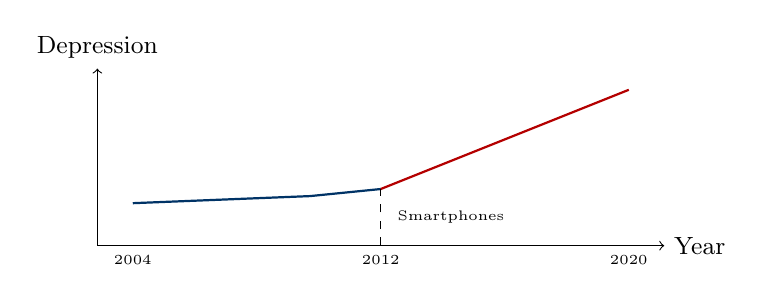
\begin{tikzpicture}[scale=0.9]
    \draw[->] (0,0) -- (8,0) node[right] {\small Year};
    \draw[->] (0,0) -- (0,2.5) node[above] {\small Depression};
    \draw[thick, aristotleblue] (0.5,0.6) -- (3,0.7) -- (4,0.8);
    \draw[thick, warningred] (4,0.8) -- (5,1.2) -- (6,1.6) -- (7.5,2.2);
    \node[below] at (0.5,0) {\tiny 2004};
    \node[below] at (4,0) {\tiny 2012};
    \node[below] at (7.5,0) {\tiny 2020};
    \draw[dashed] (4,0) -- (4,0.8);
    \node[right, font=\tiny] at (4.1,0.4) {Smartphones};
\end{tikzpicture}
\end{center}

\begin{alertblock}{?}
Have you noticed changes in your own or peers' mental health related to tech use?
\end{alertblock}
\end{frame}

% ===== SLIDE 32: Premise 2b - Commodified Relationships =====
\begin{frame}{Premise 2b: Commodification of Relationships}
\textbf{Turkle}: ``Alone Together''

\begin{itemize}
    \item \textbf{Friendship as metric}: Followers, likes, streaks
    \item \textbf{Dating apps}: Optimization and commodification of romance
    \item Loss of \textbf{serendipity} and organic connection
    \item \textbf{Parasocial relationships}: One-sided bonds with influencers/AI
    \item The \textbf{loneliness epidemic}: More ``connected'' than ever, more alone
\end{itemize}

\vspace{0.3cm}
\begin{quotebox}[Turkle]
``We expect more from technology and less from each other.''
\end{quotebox}

\begin{alertblock}{?}
How many of your online ``friends'' would you call in a genuine crisis?
\end{alertblock}
\end{frame}

% ===== SLIDE 33: Premise 2c - Distorted Self-Understanding =====
\begin{frame}{Premise 2c: Distorted Self-Understanding}
\textbf{Algorithmic identity}: You are what the algorithm thinks you are

\begin{itemize}
    \item \textbf{Filter bubbles} as distorting mirrors
    \item Algorithm shows you ``more of what you'll (predictably) pay attention to''---but is that \textit{you}?
    \item The algorithm \textbf{shapes your behavior} to maximize engagement. These might not align with your true flourishing.
\end{itemize}

\begin{center}
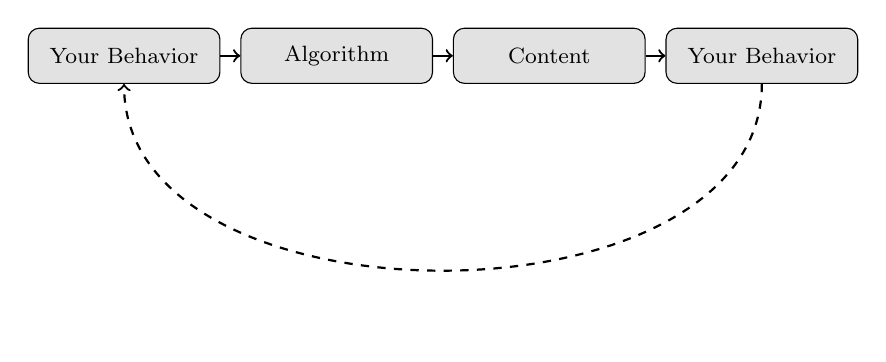
\begin{tikzpicture}[node distance=2.2cm,
    block/.style={rectangle, draw, fill=techgray!15, text width=2.2cm, text centered, rounded corners, minimum height=0.7cm, font=\footnotesize}]
    \node [block] (behavior) {Your Behavior};
    \node [block, right of=behavior, xshift=0.5cm] (algorithm) {Algorithm};
    \node [block, right of=algorithm, xshift=0.5cm] (content) {Content};
    \node [block, right of=content, xshift=0.5cm] (behavior2) {Your Behavior};
    \draw[->, thick] (behavior) -- (algorithm);
    \draw[->, thick] (algorithm) -- (content);
    \draw[->, thick] (content) -- (behavior2);
    \draw[->, thick, dashed] (behavior2.south) to[out=-90,in=-90] (behavior.south);
\end{tikzpicture}
\end{center}

\begin{alertblock}{?}
\small
Does your ``For You'' page reflect who you really are---or who the algorithm wants you to be?
\end{alertblock}
\end{frame}

% ===== PART V HEADER =====
\begin{frame}
\begin{center}
{\Huge \textbf{Part V}}\\[0.5cm]
{\Large Policy Responses}\\[0.3cm]
{\large From Diagnosis to Action}
\end{center}
\end{frame}

% ===== SLIDE 34: From Diagnosis to Policy =====
\begin{frame}{From Diagnosis to Policy}
If the virtue ethics diagnosis is correct, what follows?

\begin{itemize}
    \item \textbf{Individual responses}: Digital detox, mindfulness, intentional use
    \item \textbf{Structural responses}: Regulation, design mandates, education
    \item Virtue ethics case for regulation: Creating environments \textbf{conducive to flourishing}
\end{itemize}

\vspace{0.3cm}
\begin{table}[h]
\centering
\small
\begin{tabular}{>{\bfseries}l p{4cm} p{4cm}}
\toprule
& \textbf{Individual} & \textbf{Structural} \\
\midrule
Advantages & Personal agency, immediate & Addresses root causes \\
Limits & Willpower exhaustion, inequality & Paternalism concerns \\
Examples & Phone-free meals & Age restrictions \\
\bottomrule
\end{tabular}
\end{table}

\begin{alertblock}{?}
Is changing individual behavior enough, or do we need systemic/policy changes?
\end{alertblock}
\end{frame}

% ===== SLIDE 35: Policy Proposals =====
\begin{frame}{Policy Proposals}
\begin{block}{Australia's Social Media Minimum Age Law (2024)}
Minimum age of \textbf{16} for social media accounts; platforms face fines for non-compliance. Implemented 2025.
\end{block}

\vspace{0.2cm}
\begin{table}[h]
\centering
\small
\begin{tabular}{>{\bfseries}l p{6cm}}
\toprule
Policy Type & Virtue Ethics Rationale \\
\midrule
Age restrictions & Protect developing capacity for virtue \\
Design mandates & Remove features that habituate vice \\
Algorithm transparency & Enable informed choice \\
Digital literacy education & Cultivate technomoral wisdom \\
AI governance & Preserve authentic human connection \\
\bottomrule
\end{tabular}
\end{table}

\begin{alertblock}{?}
Should governments regulate social media to protect flourishing, or is this overreach?
\end{alertblock}
\end{frame}

% ===== SLIDE 36: Vallor's Vision =====
\begin{frame}{Vallor's Vision: Cultivating Technomoral Wisdom}
Technology as \textbf{pharmakon} (Greek: both poison and cure):

\begin{itemize}
    \item Technology can cultivate virtue \textit{or} vice---depends on design and use
    \item Need \textbf{intentional design} for virtue cultivation
    \item Need \textbf{individual practices} that build character
\end{itemize}

\vspace{0.3cm}
\begin{block}{Practical Recommendations}
\begin{itemize}
    \item \textbf{Digital sabbaths}: Regular disconnection for reflection
    \item \textbf{Attention training}: Meditation, deep reading practices
    \item \textbf{Face-to-face priority}: Protect in-person relationships
    \item \textbf{Critical consumption}: Question algorithmic recommendations
    \item \textbf{Moral ``operating systems''}: Explicit frameworks for tech use
\end{itemize}
\end{block}

\begin{alertblock}{?}
Which of these recommendations could you realistically implement this week?
\end{alertblock}
\end{frame}

% ===== PART VI HEADER =====
\begin{frame}
\begin{center}
{\Huge \textbf{Part VI}}\\[0.5cm]
{\Large Objections to Virtue Ethics}\\[0.3cm]
{\large The Critics Respond}
\end{center}
\end{frame}

% ===== SLIDE 37: Objection 1 - Positive Liberty =====
\begin{frame}{Objection 1: The Positive Liberty Problem}
\begin{objectionbox}[Berlin/Mill: The Paternalism Worry]
\small
\begin{enumerate}
    \item Virtue ethics assumes a \textbf{particular conception of the good life}.
    \item In a pluralistic society, the state should not impose any conception of the good (\textbf{negative liberty}).
    \item Restricting social media treats citizens as children unable to choose their own good.
    \item[\textbf{C.}] This is \textbf{paternalistic overreach} that threatens individual liberty.
\end{enumerate}
\end{objectionbox}

\begin{quotebox}[Isaiah Berlin, ``Two Concepts of Liberty'']
\small ``Positive liberty''---the freedom \textit{to} flourish---has historically been used to justify tyranny in the name of people's ``true'' interests.
\end{quotebox}

\begin{alertblock}{?}
Is there a meaningful difference between protecting children and ``protecting'' adults?
\end{alertblock}
\end{frame}

% ===== SLIDE 38: Responses to Liberty Objection =====
\begin{frame}{Responses to the Liberty Objection}
\begin{enumerate}
    \item \textbf{Children vs. adults}: Age-based restrictions less controversial
    
    \item \textbf{Addiction and autonomy}: Can you freely choose what undermines your capacity to choose?
    
    \item \textbf{Market failures}: ``Choice architecture'' already manipulated by corporations seeking profit
    
    \item \textbf{Harm to others}: Externalities of social media on democratic discourse
    
    \item \textbf{Soft vs. hard paternalism}: Nudges and defaults vs. outright bans
\end{enumerate}

\vspace{0.3cm}
\begin{alertblock}{Key Question}
Is it ``freedom'' to be manipulated by algorithms designed to maximize engagement at the expense of your wellbeing?
\end{alertblock}
\end{frame}

% ===== SLIDE 39: Objection 2 - Nietzsche =====
\begin{frame}{Objection 2: The Nietzschean Worry}
\begin{objectionbox}[Nietzsche: Who Decides What Virtue Is?]
\small
\begin{enumerate}
    \item Virtue ethics assumes we can reliably identify virtue vs. vice.
    \item But historical ``virtues'' often reflected \textbf{power structures} or ``\textbf{herd mentality}.''
    \item Some ``vices'' (pride, aggression) may be \textbf{necessary for excellence}.
    \item[\textbf{C.}] The virtue critique of technology may reflect \textbf{conservative bias}.
\end{enumerate}
\end{objectionbox}

\begin{quotebox}[Nietzsche, Beyond Good and Evil]
\small ``What is called virtue in the herd-man would be vice for the higher man. \ldots\ The virtues of the common man would perhaps signify vices and weaknesses in a philosopher.''
\end{quotebox}

\begin{alertblock}{?}
Could ``doom-scrolling'' ever be reframed as a virtue? What would that require?
\end{alertblock}
\end{frame}

% ===== SLIDE 40: Responses and Conclusion =====
\begin{frame}{Responses and Conclusion}
\textbf{Responses to Nietzsche}:
\begin{itemize}
    \item \textbf{Empirical grounding}: Mental health data, not just ``values''
    \item \textbf{Aristotelian $\neq$ Victorian}: Different conception of virtue
    \item Virtue ethics can be \textbf{critical tool} (challenges existing norms too)
    \item The question isn't ``Is change bad?'' but ``Does this change serve human flourishing?''
\end{itemize}

\vspace{0.3cm}
\begin{block}{Final Reflection}
The question remains genuinely open. But virtue ethics gives us a powerful framework for asking it:

\vspace{0.2cm}
\centering
\textbf{What kind of people are we becoming---and is that what we want?}
\end{block}

\vspace{0.2cm}
\small
\textbf{Discussion}: What practices in your own technological life cultivate virtue? Vice?
\end{frame}

\end{document}